\documentclass[tikz]{standalone}

\usepackage{amsmath}
\usepackage{physics}

\usetikzlibrary{arrows.meta,positioning}

\begin{document}
	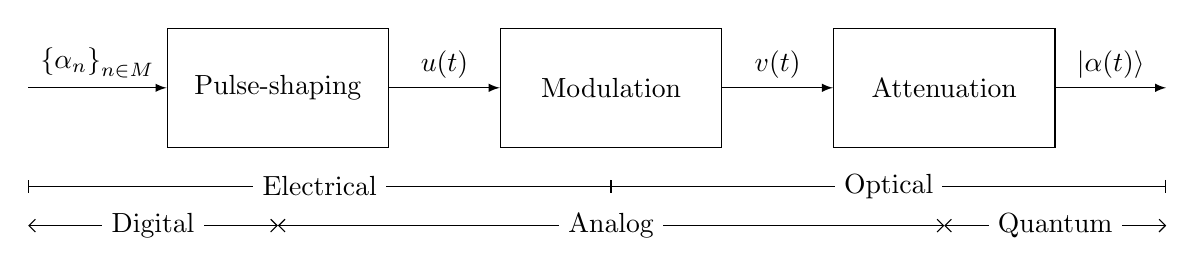
\begin{tikzpicture}[
		node distance=4em,
		arrow/.style={-latex},
		block/.style={draw, minimum height=10ex, minimum width=8em, align=center},
	]
		\coordinate (in) at (0,0);
		\node (psh) [block, right=5em of in] {Pulse-shaping};
		\node (mod) [block, right=of psh] {Modulation};
		\node (att) [block, right=of mod] {Attenuation};
		\coordinate[right=of att] (out);
		
		\draw[arrow] (in) -- node[above]{$\left\{\alpha_n\right\}_{n\in M}$} (psh);
		\draw[arrow] (psh) -- node[above]{$u(t)$} (mod);
		\draw[arrow] (mod) -- node[above]{$v(t)$} (att);
		\draw[arrow] (att) -- node[above]{$\ket{\alpha(t)}$} (out);
		
		\coordinate (eo) at (0,-1.25);
		\draw[Bar-Bar] (eo) -- (eo-|mod.south) node[midway, sloped, fill=white] {Electrical};
		\draw[Bar-Bar] (eo-|mod.south) -- (eo-|out) node[midway, sloped, fill=white] {Optical};

		\coordinate (da) at (0,-1.75);
		\draw[Straight Barb-Straight Barb] (da) -- (da-|psh.south) node[midway, sloped, fill=white] {Digital};
		\draw[Straight Barb-Straight Barb] (da-|psh.south) -- (da-|att.south) node[midway, sloped, fill=white] {Analog};
		\draw[Straight Barb-Straight Barb] (da-|att.south) -- (da-|out) node[midway, sloped, fill=white] {Quantum};
	\end{tikzpicture}
\end{document}
